\chapter{Numerical model}\label{chapter:numericalmodel}
\thispagestyle{empty}

The numerical model for CO\textsubscript{2} density-driven dissolution in water was developed by 
\citet{Class2020}. As part of the thesis, we added source and sink terms in the continuity equation 
to the  model implemented by \citet{Class2020} for modeling dissolution of calcite. We implemented 
reactive source/sink terms in the model, and for this, we sought help from \citet{hommel2016modeling} dissertation. 
A fluid system was created to suit one phase (liquid), three components (\ce{H2O}, TIC, and calcium). 
Fluid systems in \DuMuX explain the thermodynamic properties of quantities (in our model, the quantities are 
\ce{H2O, TIC} and calcium) and the relationship with each another. A two-dimensional model domain [5 mm $\times$ 15 mm] 
was setup in \DuMuX to run the simulation.

\section{Solving the reactive model}
Two tools were used to model the calcite dissolution: \MATLAB and \DuMuX. \MATLAB allowed easy testing of the 
calcite dissolution model we envisaged without the overhead of \DuMuX.

\subsection{\MATLAB} \label{ssec:matlabIntro}
\MATLAB was used to model calcite dissolution. We solved charge balance equation (\Cref{eq:chargebalfinal}) 
to calculate the rate of calcite dissolution; and the steady-state concentration of hydrogen (pH), carbonate and bicarbonate, 
calcium, and total inorganic carbon. we considered batch volume approach having only one cell of size [5 mm$\times$15 mm], 
the same model size as in \DuMuX , which would make the dissolved products instantly mix throughout the domain as 
the dissolution proceeds. In \MATLAB we solved for a closed system without outflow or inflow of calcium, TIC and water. 
We set an initial concentration of total inorganic carbon throughout the domain and started the simulation with an initial pH. 
We varied the initial pH, as mentioned in \Cref{tab:scenarios}, to understand its dependency on the rate of dissolution and 
steady-state concentrations (hydrogen, carbonate, bicarbonate, calcium, and TIC). The results that we got from \MATLAB were 
also used to validate the results from \DuMuX, as we set an identical initial and boundary conditions and a domain with just 
one cell of size [5 mm$\times$15 mm] in \DuMuX to mimic the batch volume approach adopted in \MATLAB. We expect the results 
to be identical from the \MATLAB and \DuMuX models with these setups. \\

\subsection{\DuMuX} \label{ssec:DumuxIntro}
In \DuMuX, the continuity equation (\Cref{eq:contiEq}) was solved together with the source and sink terms accounting for 
TIC and calcium. A few batch scenarios with varying parameters -- such as Initial pH; reactive-area/batch volume, if it's a closed system; 
flow-velocity, if it's an open system; \ce{CO2} concentration above the epiphreatic karst water table, if it's an open system; and grid grading 
parameter for an open system (\Cref{chapter:results}) -- were set up in \DuMuX as illustrated in \Cref{tab:scenarios}. 
\begin{enumerate}
    \item \textbf{Closed System:} The top and bottom boundary 
    conditions were set to Neumann no-flow for the fluxes across the boundary. The model domain of size [5 mm$\times$15 mm] had 
    10 divisions on the x-axis and 20 divisions on the y-axis. Initial pH, and reactive-area/batch-volume 
    were varied to understand its dependency on the rate of dissolution and steady-state concentrations (hydrogen, carbonate, bicarbonate, calcium, and TIC). \\
    For a plausible comparison with the \MATLAB results, spatial discretization was readjusted having just one cell of size [5 mm$\times$15 mm], 
    similar to the model setup in \MATLAB.

    \item \textbf{Open system:} Neumann no-flow boundary conditions were lifted, the number of grids is 10 on the x-axis and 20 on the y-axis, 
    and  protruding \ce{CO2} fingers into the karst water were set to model cave scenario. Initial pH, flow-velocity/velocity of fingers, \ce{CO2} 
    concentration above the epiphreatic karst water table and grid grading parameter were varied to understand its dependency on the rate 
    of dissolution and steady-state concentrations (hydrogen, carbonate, bicarbonate, calcium, and TIC).
\end{enumerate}


\section{Implementation in \MATLAB}
Varying initial pH of the solution and reactive-area/batch-volume, the rate of dissolution and steady-state time and 
concentrations of hydrogen, carbonate, bicarbonate, calcium and TIC were calculated. \Cref{eq:rDiss,eq:omega} were solved 
to calculate the rate of calcite dissolution (\ce{r_{diss}}). Rate of calcite dissolution when multiplied with the reactive-area 
and the time-step would give the amount of produced TIC and calcium. With the increase in calcium concentration in the 
solution, total inorganic carbon would also increase by the same amount (\ce{m^{TIC}} = $\mathrm{m_{initial}^{TIC}}$ + \ce{m^{\ce{Ca^{2+}}}}). 
Charge balance equation (\Cref{eq:chargebalfinal}) was solved for concentration of hydrogen ($\mathrm{m^{H^{+}}}$) with the updated concentrations 
of calcium and total inorganic carbon. The charge balance equation is a non-linear equation in $\mathrm{m^{H^+}}$. 
We used \MATLAB function \say{vpasolve}, a non-linear solver, to solve \Cref{eq:chargebalfinal} for $\mathrm{m^{H^+}}$. With the new 
concentration of hydrogen, rate of dissolution was calculated again for the next time-step and the cycle is repeated until it 
reaches the end of simulation. The flowchart presented in \Cref{fig:flowchartMATLAB} shows the work flow. 

\begin{center}
% \newpage
% \centering
\begin{tikzpicture}[node distance=2cm]
\node (func1) [startstop] {Start};

\node (func2) [process, below of=func1, yshift=-0.7cm] {Define all the constants including initial pH of the system and 
initial concentration of total inorganic carbon. Initialize vectors of size equal to the number of time steps to store pH, 
$\mathrm{m^{Ca^{2+}}}$, $\mathrm{m^{TIC}}$, $\mathrm{m^{{CO_3}^{2-}}}$, $\mathrm{r_{diss}}$};

\node (func3) [process, below of=func2, yshift=-1.2cm] {$\mathrm{m^{H^+} = 10^{-initial pH}}$\\
Initialize $\mathrm{m^{Ca^{2+}}}$ = 0 (no dissolution at the start of the simulation)};

\node (func4) [process, below of=func3, yshift=-1.90cm] {Calculate mCorrection \[\begin{aligned}[t]& \ce{mCorrection} = -2\ce{m^{Ca^{2+}}}\\
&+ \frac{2\ce{m^{TIC}}}{\frac{\left(\ce{m^{\ce{H^{+}}}}\right)^2}{\ce{k_{diss,1}} \cdot \ce{k_{diss,2}}}+\frac{\ce{m^{\ce{H^{+}}}}}{\ce{k_{diss,2}}} + 1} \\
&+ \frac{\ce{m^{TIC}}}{\frac{\ce{m^{\ce{H^{+}}}}}{\ce{k_{diss,1}}} + 1 + \frac{\ce{k_{diss,2}}}{\ce{m^{\ce{H^{+}}}}}} - \ce{m^{\ce{H^{+}}}} + 
\frac{\ce{K_w}}{\ce{m^{\ce{H^{+}}}}}.\end{aligned}\]};

\node (conn1) [connector, below of=func4, yshift=-1.5cm] {A};


% lines
\path [line] (func1) -- (func2);
\path [line] (func2) -- (func3);
\path [line] (func3) -- (func4);
\path [line] (func4) -- (conn1);

\end{tikzpicture}
\end{center}

\begin{figure}
\newpage
\centering
\begin{tikzpicture}[node distance=2cm]
\centering
\node (conn1) [connector] {A};

\node (func5) [process, below of=conn1] {save pH, $\mathrm{m^{Ca^{2+}}}$ and $\mathrm{m^{TIC}}$ to their respective vectors};

\node (func6) [process, below of=func5, yshift=-2.0cm] {Solve charge balance equation (\Cref{eq:chargebalfinal}) for \ce{m^{\ce{H^+}}}\[\begin{aligned}[t]
&2\ce{m^{Ca^{2+}}} - \frac{2\ce{m^{TIC}}}{\frac{\left(\ce{m^{\ce{H^{+}}}}\right)^2}{\ce{k_{diss,1}} \cdot \ce{k_{diss,2}}}+1+\frac{\ce{m^{\ce{H^{+}}}}}
{\ce{k_{diss,2}}}}\\
&- \frac{\ce{m^{TIC}}}{\frac{\ce{m^{\ce{H^{+}}}}}{\ce{k_{diss,1}}}+1+\frac{\ce{k_{diss,2}}}{\ce{m^{\ce{H^{+}}}}}} + \ce{m^{\ce{H^{+}}}} - 
\frac{\ce{K_w}}{\ce{m^{\ce{H^{+}}}}}\\
&+ \ce{mCorrection} = 0. \end{aligned}\]};

\node (func7) [process, below of=func6, yshift=-2.2cm] {Calculate $\mathrm{m^{CO_3^{2-}}}$ = $\frac{\ce{m^{TIC}}}{\frac{\left(\ce{m^{\ce{H^{+}}}}
\right)^2}{\ce{k_{diss,1}} \cdot \ce{k_{diss,2}}}+1+\frac{\ce{m^{\ce{H^{+}}}}}{\ce{k_{diss,2}}}}$\\ and save to its vector};

\node (func8) [process, below of=func7, yshift=-0.3cm] {Calculate Omega = $\mathrm{m^{Ca^{2+}}}$ * $\mathrm{m^{CO_3^{2-}}}$/$\mathrm{K_{sp}}$.};

\node (func9) [process, below of=func8, yshift=-0.0cm]  {Save Omega to its vector and initialize \ce{r_{diss}} = 0.};

\node (dec2) [decision, below of=func9, yshift=-1.2cm] {Omega $<$ 1};

\node (conn3) [connector, below of=dec2, yshift=-1.5cm] {A};

\node (conn4) [connector, right of=conn3, xshift=3cm] {C};

\node (conn5) [connector, right of=conn3, xshift=5cm] {B};

% lines
\path [line] (conn1) -- (func5);
\path [line] (func5) -- (func6);
\path [line] (func6) -- (func7);
\path [line] (func7) -- (func8);
\path [line] (func8) -- (func9);
\path [line] (func9) -- (dec2);
\path [line] (dec2) -- node[anchor=east]{yes}(conn3);
\path [line] (dec2) -| node[anchor=south]{no}(conn4);
\path [line] (conn5) |- (func5);

\end{tikzpicture}
\end{figure}

\begin{figure}
\newpage
\centering
\begin{tikzpicture}[node distance=2cm]

\node (conn1) [connector] {A};

\node (conn2) [connector, right of=conn1, xshift=5cm] {B};
\node (conn3) [connector, right of=conn1, xshift=3cm] {C};

\node (func10) [process, below of=conn1, yshift=-0.0cm] {$\mathrm{r_{diss}}$ = $\mathrm{(k_{diss,1} * m^{H^+} + k_{diss,2}) * (1 - Omega)}$.};

\node (func11) [process, below of=func10, yshift=-0.0cm] {save \ce{r_{diss}} to a vector};

\node (func12) [process, below of=func11, yshift=-0.5cm] {Calculate new calcium concentration\\
$\Delta \mathrm{m^{Ca^{2+}}} = \mathrm{r_{diss}}$ * Time-step * Reactive-area, \\
$\mathrm{m^{Ca^{2+}}} = \mathrm{m^{Ca^{2+}}} + \frac{\Delta\mathrm{m^{Ca^{2+}}}}{\ce{Batch volume} * \rho}$.};

\node (func13) [process, below of=func12, yshift=-0.5cm] {Update $\mathrm{m^{TIC}} = \mathrm{m_{initial}^{TIC}} + \mathrm{m^{Ca^{2+}}}$.};

\node (dec1) [decision, below of=func13, yshift=-1.5cm] {check for the end of simulation};



\node (func14) [startstop, below of=dec1, yshift=-1.5cm] {End};
% lines
\path [line] (conn1) -- (func10);
\path [line] (func10) -- (func11);
\path [line] (func11) -- (func12);
\path [line] (func12) -- (func13);
\path [line] (func13) -- (dec1);
\path [line] (dec1) -- node[anchor=east]{yes}(func14);
\path [line] (conn3) |- (func11);
\path [line] (dec1) -| node[anchor=north]{no}(conn2);

\end{tikzpicture}
\caption [Flowchart for the workflow in \MATLAB] {\textbf{Flowchart for the workflow in \MATLAB}}
\label{fig:flowchartMATLAB}
\end{figure}

\newpage
\section{Implementation in \DuMuX}\label{ssec:impdum}
The numerical simulator \DuMuX helps us to solve complex differential equations as we encounter in free/porous medium flow. 
We use the \textit{freeflow Navier-Stokes model} in \DuMuX and employ \textit{h2oco2calcium} fluid system. 
The fluid-system had one phase (liquid phase) and three components (\ce{H2O, TIC, calcium}). We only considered the density 
of water in calculating the density of the fluid. We also switched-off the gravity and assumed a constant hydro-static pressure 
throughout the domain of size [5 mm $\times$ 15 mm]. Given the size of the domain, assuming a constant hydro-static pressure was 
a reasonable assumption, as this made the model less sophisticated to implement the reactive source and sink terms, which was our 
primary goal. Nevertheless, for modeling bigger geological systems, gravity cannot be switched off as there 
will be a significant rise in the pressure as the depth increases.\\
We used a staggered-grid, finite volume method for solving primary variables in every control volume. 
All equations are solved implicitly using Newton solver. The Newton solver adapts 
the time step size depending on the convergence of the solution and is limited by a user-controlled maximum time-step size. 
For further information on discretization, numerical methods and it's implementation, refer to \cite{Koch2020} or the handbook 
of \DuMuX \cite{Kochetal2020Dumux}.

\subsection{Primary variables} Pressure and concentration  of TIC, calcium and \ce{H2O}, three scalar variables, in 
terms of mole fraction, as well as, the velocity vector were selected as primary unknowns. 

\subsection{Boundary conditions} 
The velocity vector ($\mathbf{v}$), pressure (p) and the concentrations of TIC and calcium are set to Dirichlet values; 
and \ce{H2O}, TIC and calcium fluxes are set to Neumann values in the NS-model. We had two setups in \DuMuX i.e., open 
and closed systems, and boundary conditions were different for these two setups. Flowchart in \Cref{sec:flowChartBC} shows boundary 
condition implementation in \DuMuX. 

\paragraph*{Open system} \mbox{} \\

As shown in \Cref{fig:OpenedSystem}, we set Dirichlet condition at the top boundary for velocities in x and y directions 
and concentration of TIC and calcium. For the left boundary, we assumed no-slip condition as we set Dirichlet condition for 
velocities and Neumann condition for TIC and calcium fluxes. Similarly, for the bottom boundary Dirichlet condition was set 
for pressure and Outflow conditions for TIC and calcium fluxes formed due to the dissolution of calcite. we set Symmetric property 
at the right boundary instead of assigning identical left boundary conditions that also reduced the computational time.

\begin{figure}
    \centering
    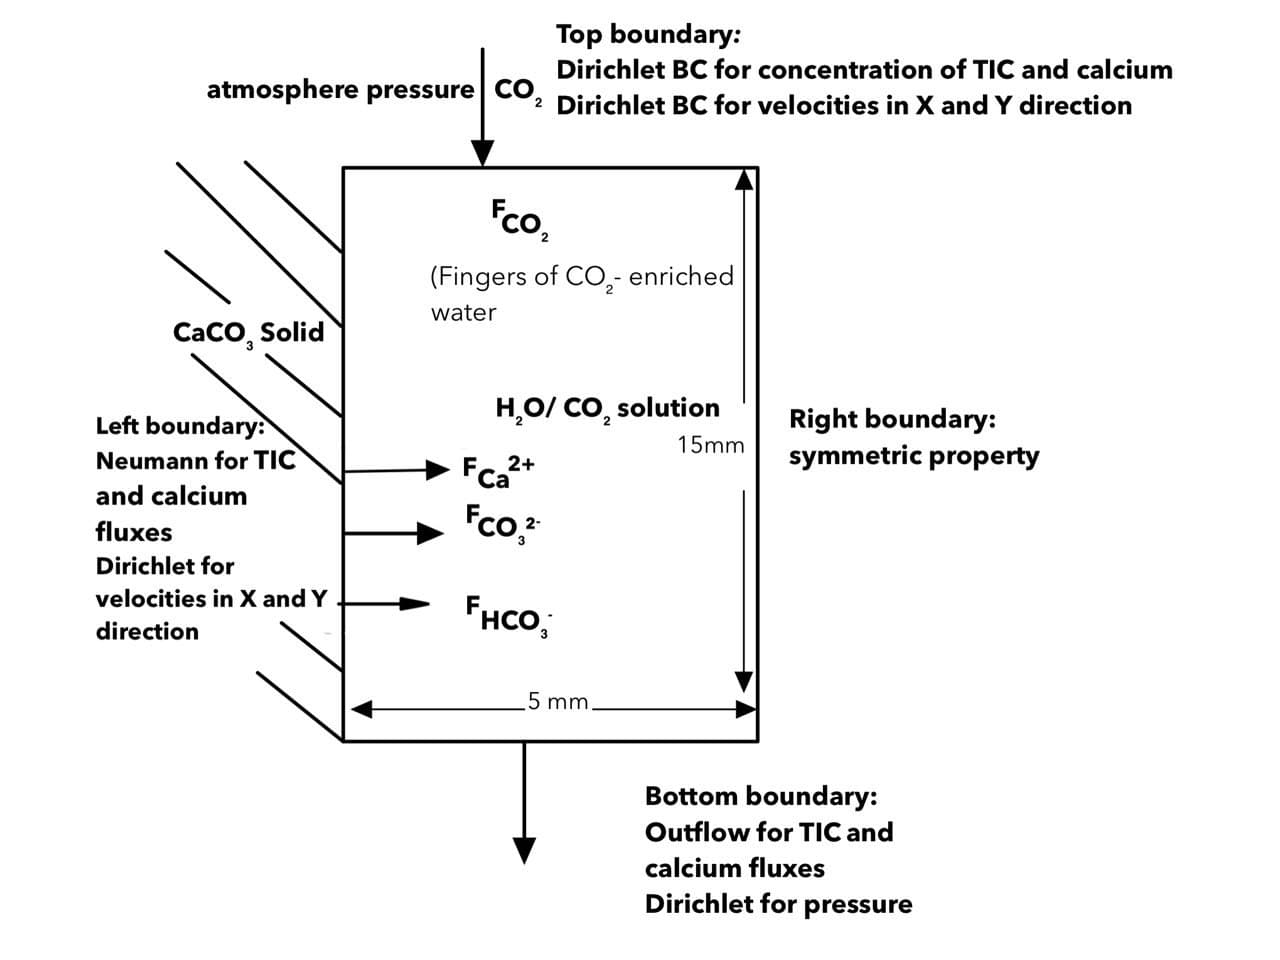
\includegraphics[width=0.75\textwidth]{PICTURES/opened_system.jpg}
    \caption [Model domain and boundary conditions for \ce{CaCO3} dissolution in an open system] {\textbf{Model domain and boundary conditions for \ce{CaCO3} dissolution in an open system}}
    \label{fig:OpenedSystem}       % Give a unique label
\end{figure}


\paragraph*{Closed system} \mbox{} \\
As shown in \Cref{fig:ClosedSystem}, we set Dirichlet condition at the top boundary for velocities in x and y direction and 
Neumann no-flow for TIC and calcium fluxes. For the left boundary, we assumed no-slip condition -- similar 
to the open system -- as we set Dirichlet condition for velocities and Neumann condition for TIC and calcium fluxes. On the 
bottom boundary, we set Dirichlet condition for pressure and Neumann no-flow for TIC and calcium fluxes. 
We also set symmetric property at the right boundary -- again, similar to the open system. Hence, the only difference between 
these two setups was the top and bottom boundary conditions. 

\begin{figure}
    \centering
    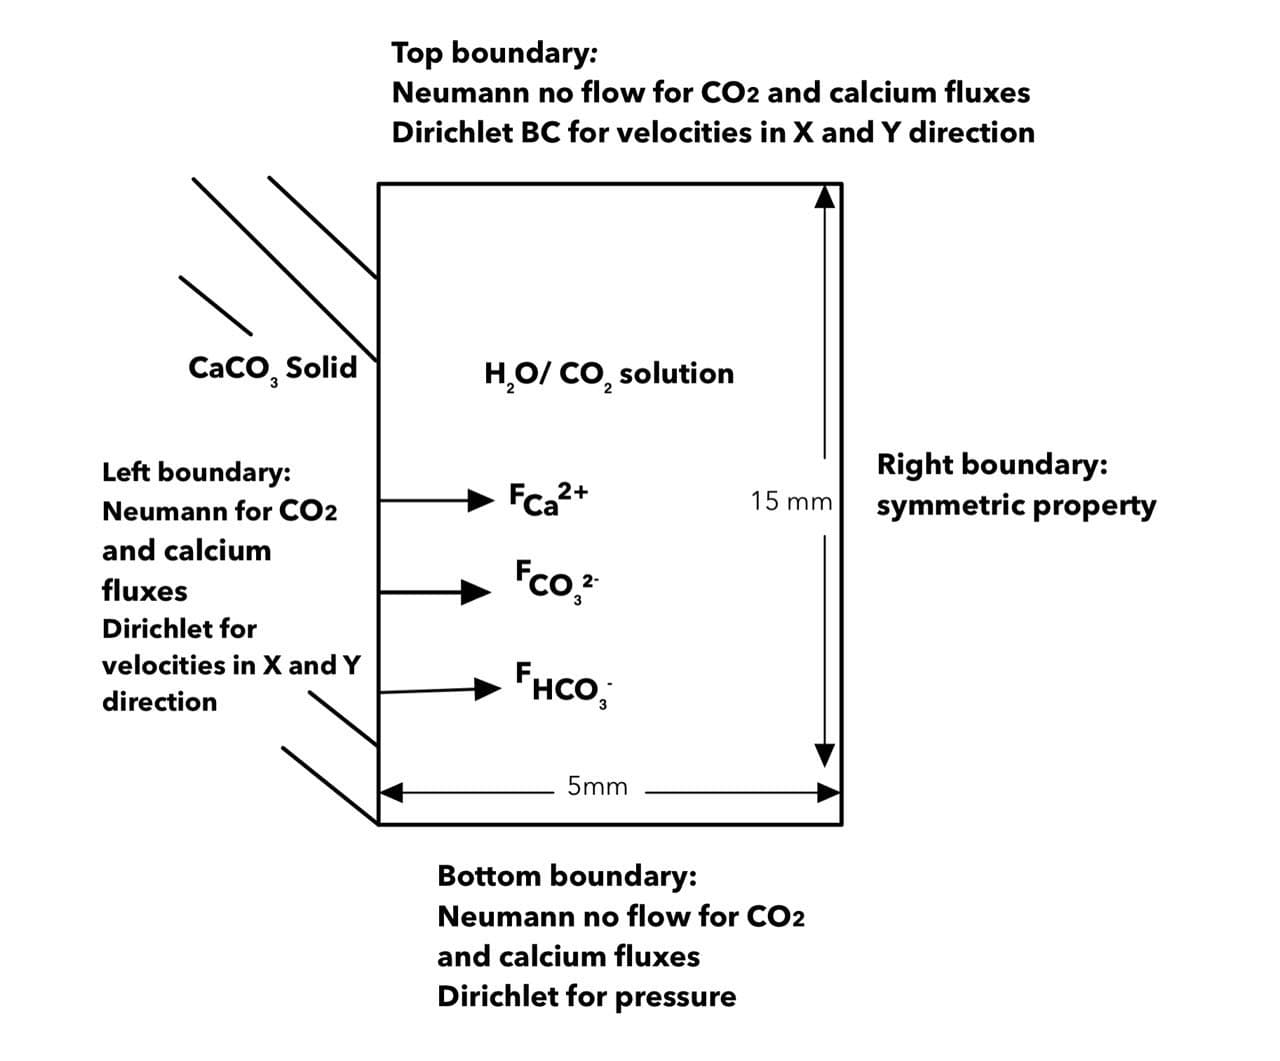
\includegraphics[width=0.75\textwidth]{PICTURES/closed_system.jpg}
    \caption [Model domain and boundary conditions for \ce{CaCO3} dissolution in a closed system] {\textbf{Model domain and boundary conditions for \ce{CaCO3} dissolution in a closed system}}
    \label{fig:ClosedSystem}       % Give a unique label
\end{figure}
 

\subsection{Source/Sink term} A function, \code{reactionSource()}, was implemented which calculates the added concentration of 
TIC and calcium into the solution because of the dissolution of calcite. On the one hand addition of \ce{CO2} in karst water in an open system 
reduces the pH, on the other hand addition of carbonic acid replenishes the dissolution potential of the karst water used up  
during the dissolution of calcite, thereby sustaining dissolution of calcite and forming carbonates and bicarbonates which increases the pH. 
Therefore, steady-state is expected to be dependent on the flow-velocity with which \ce{CO2} is being carried into the karst water 
and adjusted to new acidity and consequence alkalinity. Unlike in an open system, carbonic acid in a closed system does not get 
replenished; hence, the rate of dissolution would eventually come to naught at the steady-state. 


\subsection{Solving reaction equation} A function, \code{setValues()}, calls \code{calculateValues\_()} function that solves the charge 
balance equation (\Cref{eq:chargebalfinal}) for a given time step throughout the domain and saves the calculated values to a vector. 
The saved values were then retrieved and used for visualization in Paraview \cite{ahrens2005paraview}. The function \code{reactionSource()} needs molality of 
hydrogen ($\mathrm{m^{H^+}}$), which is already calculated and stored in a vector, to calculate the added concentration of TIC 
and calcium into the solution due to dissolution of calcite. \\
The charge balance equation was solved for $\mathrm{m^{H^+}}$ using Brent's algorithm \cite{brent1971algorithm} -- a non-linear solver 
for finding root of a scalar function. 


Flowchart in \Cref{fig:flowchartReactionSource} shows the reaction source function's implementation and flowcharts in \Cref{app:appendixA} 
shows further implementations in \DuMuX.

\begin{figure}
\newpage
\centering
\begin{tikzpicture}[node distance=2cm]
\centering
\node (func1) [predefinedprocess] {\code{reactionSource} function};

\node (pro1) [process, below of=func1, yshift=-0.0cm] {Extract pH stored in its vector and calculate \[\mathrm{m^{H^+} = 10^{-pH}}\]};

\node (pro2) [process, below of=pro1, yshift=-0.5cm] {Retrieve the values $\mathrm{m^{Ca^{2+}}}$ and $\mathrm{m^{TIC}}$ from volume variables};

\node (pro3) [process, below of=pro2, yshift=-0.5cm] {Calculate $\mathrm{m^{CO_3^{2-}}}$ = $\frac{\ce{m^{TIC}}}
{\frac{\left(\ce{m^{\ce{H^{+}}}}\right)^2}{\ce{k_{diss,1}} \cdot \ce{k_{diss,2}}}+1+\frac{\ce{m^{\ce{H^{+}}}}}{\ce{k_{diss,2}}}}$};

\node (pro4) [process, below of=pro3, yshift=-0.8cm] {Calculate Omega = $\mathrm{m^{Ca^{2+}}}$ * $\mathrm{m^{CO_3^{2-}}}$/$\mathrm{K_{sp}}$.};

\node (pro5) [process, below of=pro4, yshift=-0.3cm] {Initialize \ce{r_{diss}} = 0};

\node (dec1) [decision, below of=pro5, yshift=-1cm] {Omega $<$ 1.0};

\node (pro6) [process, right of=dec1, xshift=5cm] {$\mathrm{r_{diss}}$ = $\mathrm{(k_{diss,1} * m^{H^+} + k_{diss,2}) * (1 - Omega)}$.};

\node (pro7) [process, below of=dec1, yshift=-2.0cm] {Calculate the source terms for TIC and calcium.
\[\ce{q^{TIC}} \code{ += } \ce{r_{diss}},\] \[\ce{q^{\ce{Ca}}} \code{ += } \ce{r_{diss}}.\]};


% lines
\path [line] (func1) -- (pro1);
\path [line] (pro1) -- (pro2);
\path [line] (pro2) -- (pro3);
\path [line] (pro3) -- (pro4);
\path [line] (pro4) -- (pro5);
\path [line] (pro5) -- (dec1);
\path [line] (dec1) -- node[anchor=east]{no}(pro7);
\path [line] (pro6) |- (pro7);
\path [line] (dec1) -- node[anchor=south]{yes}(pro6);
\end{tikzpicture}
\caption [Flowchart for reactionSource function in \DuMuX] {\textbf{Flowchart for reactionSource function in \DuMuX}}
\label{fig:flowchartReactionSource}
\end{figure}


\endinput